\documentclass[a4,12pt]{article} 
\usepackage{graphicx}
\usepackage{xepersian} 
\settextfont{Yas} 
\title{ تکالیف سری اول کنترل خطی}
\author{یاسمین خورشیدی 40117963}
\begin{document}
	\maketitle
	 در این بخش سعی میشود از عکس استفاده گردد.
	 \section{سوال اول}{
%	\begin{figure}
		\centering
%		\textbf{سوال 1 :}
		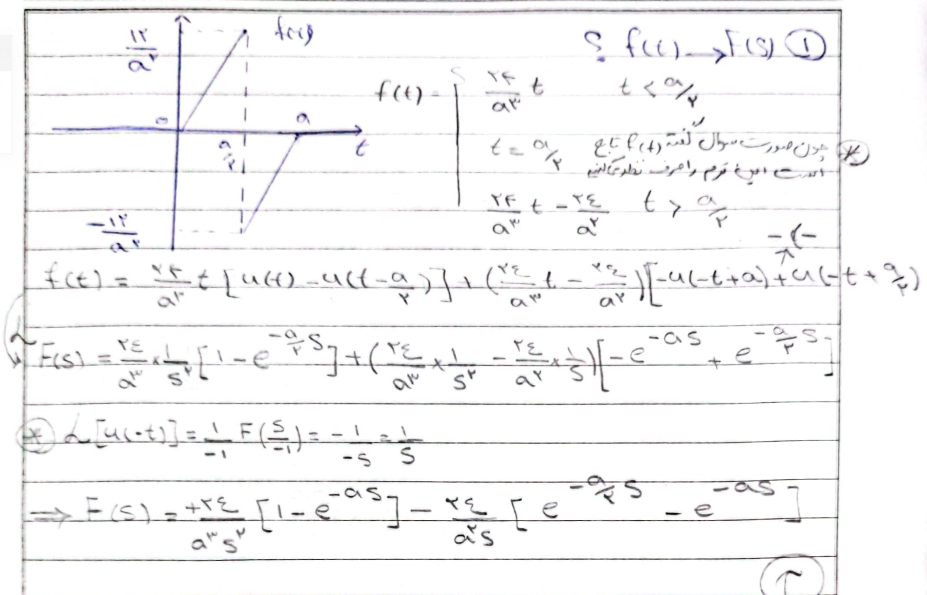
\includegraphics[width=15cm]{s1.png}
%	\end{figure}
}
   \section{سوال دوم}{
%   \begin{figure}
    	\centering   
%    	\textbf{سوال 2 :}
    	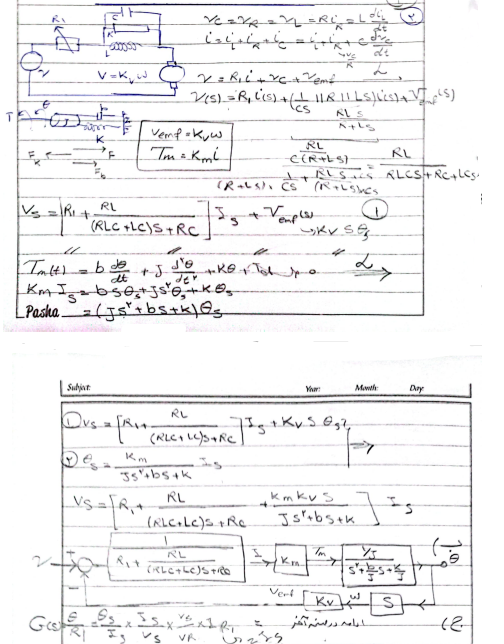
\includegraphics[width=15cm]{s21.png}\\
    	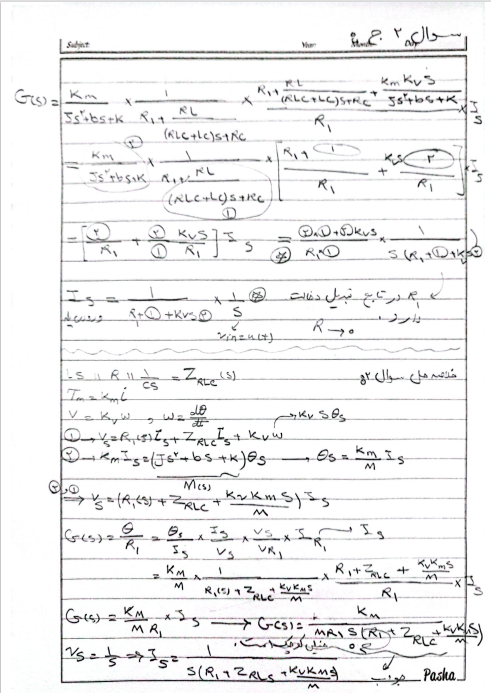
\includegraphics[width=15cm]{s22.png}
%    \end{figure}

     \section{سوال سوم}{
%    \begin{figure}
%    	\textbf{سوال 3 :}
%    	\centering
    	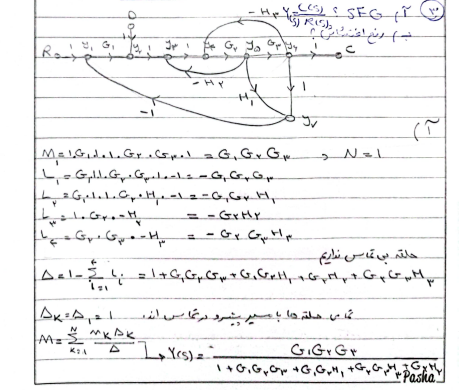
\includegraphics[width=12cm]{s31.png}
    	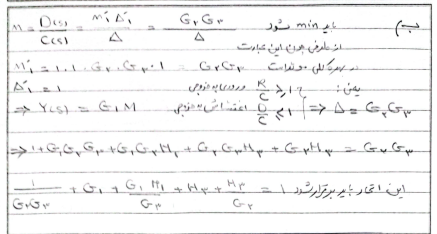
\includegraphics[width=12cm]{s32.png} 
   
 %   \end{figure}
}

     \section{سوال چهارم}{
%    \begin{figure}
%    	\textbf{سوال 4 :}   	
%    	\centering
    	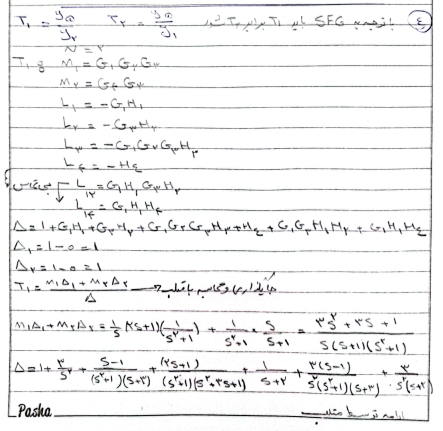
\includegraphics[width=15cm]{s4.png}
    	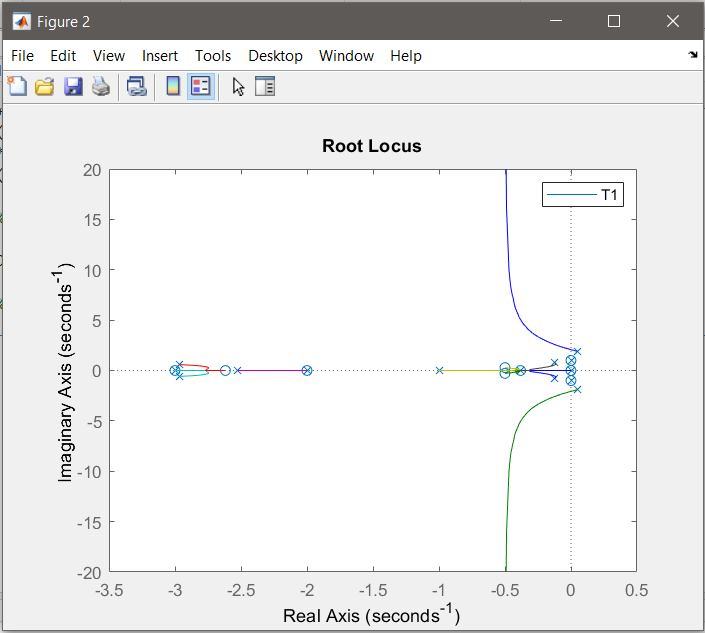
\includegraphics[width=10cm]{p41.png}
    	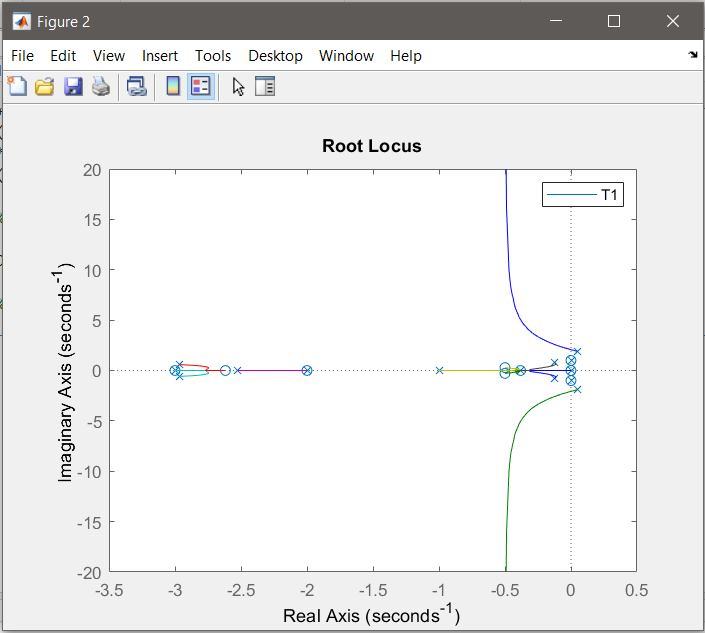
\includegraphics[width=10cm]{p41.png}
%    \end{figure}
}
\end{document}

